\documentclass[11pt,a4paper]{article}
\usepackage[T1]{fontenc}
\usepackage[utf8]{inputenc}
\usepackage[english]{babel}
\usepackage{amsmath,amssymb,mathtools,amsthm}
\usepackage{newtxtext,newtxmath,microtype}
\usepackage[a4paper,left=28mm,right=28mm,top=26mm,bottom=25mm]{geometry}
\usepackage{xcolor,booktabs,tabularx,array,longtable}
\usepackage{tikz}
\usetikzlibrary{positioning,arrows.meta,calc,babel}
\usepackage{titlesec,enumitem,fancyhdr}
\usepackage[colorlinks=true,linkcolor=InkBlue,citecolor=InkBlue,urlcolor=InkBlue]{hyperref}
\usepackage[capitalize,nameinlink,noabbrev]{cleveref}
\definecolor{InkBlue}{HTML}{203A51}
\definecolor{Copper}{HTML}{946C50}
\definecolor{Graphite}{HTML}{27323B}
\definecolor{Faint}{HTML}{687580}
\definecolor{Pale}{HTML}{EFF3F5}
\color{Graphite}
\titleformat{\section}{\Large\bfseries\color{InkBlue}}{\thesection}{0.65em}{}
\titleformat{\subsection}{\large\bfseries\color{InkBlue}}{\thesubsection}{0.65em}{}
\titlespacing*{\section}{0pt}{13pt}{6pt}
\titlespacing*{\subsection}{0pt}{10pt}{5pt}
\setlength{\parindent}{0pt}
\setlength{\parskip}{4pt}
\setlength{\emergencystretch}{2em}
\setlist[itemize]{leftmargin=17pt,topsep=3pt,itemsep=2pt}
\setlist[enumerate]{leftmargin=18pt,topsep=3pt,itemsep=3pt}
\fancyhf{}
\fancyhead[L]{\footnotesize\color{Faint}\textsc{Inheritance, seed, and functional recovery}}
\fancyhead[R]{\footnotesize\color{Faint}22 Nov 2026}
\fancyfoot[L]{\footnotesize\color{Faint}Manuscript for mathematical review}
\fancyfoot[R]{\footnotesize\color{Faint}\thepage}
\renewcommand{\headrulewidth}{0.3pt}
\pagestyle{fancy}
\newtheoremstyle{mine}{7pt}{7pt}{\normalfont}{} {\bfseries\color{InkBlue}}{.}{.5em}{}
\theoremstyle{mine}
\newtheorem{theorem}{Theorem}[section]
\newtheorem{lemma}[theorem]{Lemma}
\newtheorem{proposition}[theorem]{Proposition}
\newtheorem{corollary}[theorem]{Corollary}
\theoremstyle{definition}
\newtheorem{definition}[theorem]{Definition}
\newtheorem{remark}[theorem]{Remark}
\newcommand{\HH}{\mathcal H}
\newcommand{\WW}{\mathcal W}
\newcommand{\NN}{\mathbb N}
\newcommand{\CC}{\mathbb C}
\newcommand{\RR}{\mathbb R}
\newcommand{\norm}[1]{\left\lVert#1\right\rVert}
\newcommand{\inner}[2]{\left\langle#1,#2\right\rangle}
\newcommand{\rad}{\operatorname{rad}}
\newcommand{\dist}{\operatorname{dist}}
\newcommand{\RH}{\mathrm{RH}}
\hypersetup{pdftitle={From the inherited seed to functional recovery: a chained demonstration},pdfsubject={O58, Pell, Moebius, RA-01, and the Riemann criterion},pdfauthor={Endless Monkey Project / Relational Geometry Program}}
\begin{document}
\thispagestyle{empty}
\vspace*{8mm}
{\color{Copper}\rule{27mm}{1.7pt}}\\[14pt]
{\sffamily\small\bfseries\color{Copper} RESEARCH ARTICLE \;\textbar\; CHAINED DEMONSTRATION}\\[11pt]
{\fontsize{21}{25}\selectfont\bfseries\color{InkBlue}From the inherited seed to\\[3pt]functional recovery}\\[9pt]
{\fontsize{12.5}{17}\selectfont\color{Faint}O58, Pell recurrences, prime references, M\"obius inversion, and the Riemann criterion}\\[12pt]
{\small November 22, 2026 \;\textbar\; Version 2.1 \;\textbar\; Mathematical and editorial revision}\\[10pt]
\rule{\linewidth}{.55pt}
\vspace{3pt}
\textbf{Abstract.} A single chain of demonstrations connects the outstanding unit in O58 to an integral Pell family, the eventual incorporation of every prime reference, exact reconstruction by M\"obius inversion, and functional recovery in the Nyman--Beurling space. The following results are proved: (i) persistence of the unit seed under normalization; (ii) coverage of every squarefree index by a single inherited chain; (iii) identity of the functional spaces generated by sieve discrepancies; and (iv) exact conservation of the unit query and accounting of recovery gains. Combining these results with a published theorem of B\'aez-Duarte yields a precise equivalence: the Riemann hypothesis holds exactly when the recovered part along this particular chain tends to one. A transfer obstruction is also established: the geometric remainder $N^{-2}$ in O58 cannot uniformly bound the squared functional approximation error, in view of a classical lower bound. The equivalence organizes the problem and pinpoints its quantitative proof obligation; \textbf{it is not an unconditional proof of the Riemann hypothesis}.

\textbf{Keywords.} Seed; reference; inheritance; recoverable information; Pell; M\"obius; projection; Nyman--Beurling; Riemann.
\vspace{6pt}
\begin{center}
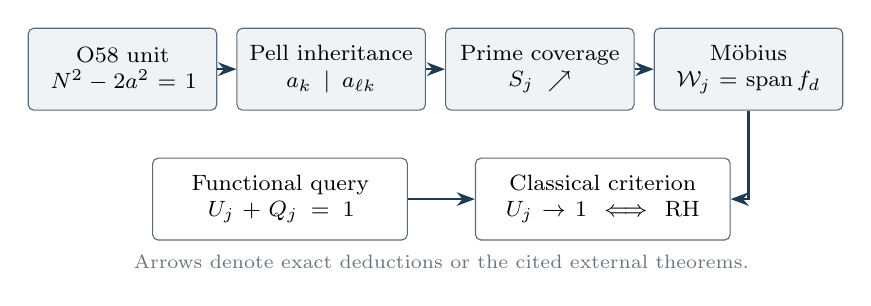
\begin{tikzpicture}[x=1cm,y=1cm,>=Stealth]
\tikzset{stage/.style={draw=InkBlue!75,rounded corners=2pt,align=center,text width=2.16cm,minimum height=1.04cm,fill=Pale,font=\footnotesize}}
\node[stage] (a) at (1.15,0) {O58 unit\\$N^2-2a^2=1$};
\node[stage] (b) at (3.80,0) {Pell inheritance\\$a_k\mid a_{\ell k}$};
\node[stage] (c) at (6.45,0) {Prime coverage\\$S_j\nearrow$};
\node[stage] (d) at (9.10,0) {M\"obius\\$\WW_j=\operatorname{span}f_d$};
\draw[->,thick,InkBlue] (a)--(b);
\draw[->,thick,InkBlue] (b)--(c);
\draw[->,thick,InkBlue] (c)--(d);
\node[stage,text width=3.0cm,fill=white] (e) at (3.15,-1.65) {Functional query\\$U_j+Q_j=1$};
\node[stage,text width=3.0cm,fill=white] (f) at (7.25,-1.65) {Classical criterion\\$U_j\to1\ \Longleftrightarrow\ \RH$};
\draw[->,thick,InkBlue] (d.south) |- (f.east);
\draw[->,thick,InkBlue] (e)--(f);
\node[font=\scriptsize,text=Faint,align=center] at (5.2,-2.45) {Arrows denote exact deductions or the cited external theorems.};
\end{tikzpicture}
\end{center}
\vfill
\rule{\linewidth}{.5pt}
{\footnotesize\color{Faint}Status: arithmetic and functional results proved under stated hypotheses; reduction to RH supported by a classical criterion; unconditional global estimate remains open.}\newpage

\section{Scope and reading conventions}

Information is defined operationally as a \emph{recoverable difference under a contract of queries}. A \emph{seed} is a recognizable and inheritable relation; \emph{normalization} expresses its relative weight at a given scale, and \emph{reclosure} consolidates admissible answers without requiring enumeration of the interior. The conditions of sufficiency, idempotence, and compositionality appear in MF--86 and CR--6 \cite{MF86,CR6}. Their meaning is contextual: a new query may require an enlarged interface.

Three objects are kept distinct throughout:
\begin{enumerate}
\item The primitive unit $1$ in the integer relation O58, which is preserved whenever a new admissible state is formed.
\item The normalized fraction $1/N^2$ of this unit at a given arithmetic scale.
\item The functional target $\chi$, normalized by $\norm\chi_2^2=1$, and its recovered component in a family of reference spaces.
\end{enumerate}

Identifying these three notions is not assumed. The argument proves the precise connections between them and exhibits a quantitative obstruction to a stronger identification.

\section{The integer seed and O58 reclosures}

\begin{definition}[Two-channel O58 contract]
An admissible state is a triple $(a,b,N)$ of positive integers satisfying
\begin{equation}\label{eq:o58}
 a^2+b^2+1=N^2.
\end{equation}
Its normalized representation is
\begin{equation}\label{eq:o58norm}
\frac{a^2}{N^2}+\frac{b^2}{N^2}+\frac1{N^2}=1.
\end{equation}
The integer $1$ is the \emph{outstanding seed}; the quotient $1/N^2$ is its representation relative to $N$.
\end{definition}

This contract comes from O58 (October 21, 2026), which explicitly separates pure rescaling from a new closure with a primitive remainder of one \cite{O58}.

\begin{lemma}[Seed continuity and distinct operations]\label{le:transport}
If $N\mid M$, $q=M/N$, and the states $(a,b,N)$ and $(a',b',M)$ both satisfy \eqref{eq:o58}, then the previous outstanding fraction transports as $1/N^2=q^2/M^2$, whereas the new primitive seed is $1/M^2$. Moreover,
\begin{equation}\label{eq:trace}
\frac{a'^2-q^2a^2}{M^2}+\frac{b'^2-q^2b^2}{M^2}+\frac{1-q^2}{M^2}=0.
\end{equation}
\end{lemma}
\begin{proof}
The transport identity follows from $M=qN$. Expressing both normalized relations over denominator $M^2$ and subtracting them proves \eqref{eq:trace}.
\end{proof}

\begin{lemma}[Infinite family of Pell reclosures]\label{le:pell}
Let
\begin{equation}\label{eq:pell}
N_k+a_k\sqrt2=(3+2\sqrt2)^k,\qquad k\ge1.
\end{equation}
Then $N_k,a_k$ are positive integers, $N_k^2-2a_k^2=1$, and $N_k\to\infty$. Therefore the symmetric branch $(a_k,a_k,N_k)$ satisfies O58, with
\begin{equation}\label{eq:seed-limit}
\frac{2a_k^2}{N_k^2}=1-\frac1{N_k^2}\longrightarrow1,
\qquad \frac1{N_k^2}\longrightarrow0.
\end{equation}
\end{lemma}
\begin{proof}
The algebraic norm of $3+2\sqrt2$ is $9-8=1$, and norm multiplicativity gives $N_k^2-2a_k^2=1$. The integer recurrence
$N_{k+1}=3N_k+4a_k$, $a_{k+1}=2N_k+3a_k$ preserves positivity. Since $3+2\sqrt2>1$ while its conjugate is below one, $N_k\to\infty$. Division by $N_k^2$ completes the proof.
\end{proof}

\begin{remark}
The limit \eqref{eq:seed-limit} does \emph{not erase} the integer $1$ in any stage's defining relation. It states that its normalized representation tends to zero. O58 proves the existence of these trajectories, but supplies no unique law choosing the next branch. The subfamily $k\mapsto3k$ also furnishes nested scales, because $N_k\mid N_{3k}$ \cite{O58}.
\end{remark}

\section{Pell inheritance and prime-reference coverage}

The arithmetic connection was developed in the \emph{Single-scale Pell audit} of November 20, 2026 \cite{PellAudit}. The argument is reproduced in full to avoid postulating any reference-incorporation step.

\begin{lemma}[Inherited divisibility]\label{le:div}
For $k,\ell\ge1$, one has $a_k\mid a_{\ell k}$.
\end{lemma}
\begin{proof}
Write $(N_k+a_k\sqrt2)^\ell=N_{\ell k}+a_{\ell k}\sqrt2$. The coefficient of $\sqrt2$ is a sum of terms involving odd powers of $a_k\sqrt2$, each divisible by the integer $a_k$.
\end{proof}

\begin{lemma}[Occurrence of every prime]\label{le:orbit}
For every prime $p$, there is an integer $1\le t_p\le p^2$ such that $p\mid a_{t_p}$.
\end{lemma}
\begin{proof}
The updating rule is
\[
\begin{pmatrix}N_{k+1}\\a_{k+1}\end{pmatrix}
=\begin{pmatrix}3&4\\2&3\end{pmatrix}
\begin{pmatrix}N_k\\a_k\end{pmatrix}.
\]
The matrix has determinant $1$ and thus induces a bijective linear transformation on the $p^2$ vectors of $\mathbb F_p^2$. The orbit of $(1,0)$ returns to its initial vector after a positive period $t_p\le p^2$. At that time the second coordinate obeys $a_{t_p}\equiv0\pmod p$.
\end{proof}

\begin{theorem}[Prime coverage by a single chain]\label{th:coverage}
Define
\begin{equation}\label{eq:chain}
\kappa_j=\operatorname{lcm}(1,\ldots,j),\quad A_j=a_{\kappa_j},
\quad S_j=\{p:\ p\text{ prime},\ p\mid A_j\}.
\end{equation}
Then $A_j\mid A_{j+1}$, $S_j\subseteq S_{j+1}$, and every positive squarefree integer divides $A_j$ from some stage onward.
\end{theorem}
\begin{proof}
Since $\kappa_j\mid\kappa_{j+1}$, \cref{le:div} gives $A_j\mid A_{j+1}$. For a prime $p$, \cref{le:orbit} provides $t_p$; whenever $j\ge t_p$, one has $t_p\mid\kappa_j$, hence $a_{t_p}\mid A_j$ and $p\in S_j$. A squarefree $d$ has finitely many prime factors, so taking a stage beyond all their thresholds proves the final assertion.
\end{proof}

This is \emph{exact coverage}. It neither bounds the construction cost polynomially nor assigns a finite physical time to the simultaneous availability of all references.

\section{From prime coverage to M\"obius queries}

Let $\mu$ be the M\"obius function, and put $\{y\}=y-\lfloor y\rfloor$. For $d\ge1$, define the fractional-part function
\begin{equation}\label{eq:fd}
f_d(x)=\left\{\frac{1}{dx}\right\}
=\frac{1}{dx}-\left\lfloor\frac{1}{dx}\right\rfloor,\qquad x>0.
\end{equation}
Thus $f_d(x)$ is exactly the fractional part of $1/(dx)$. For a finite set $S$ of primes let $M_S:=\prod_{p\in S}p$, with $M_\varnothing=1$. The corresponding sieve discrepancy is
\begin{equation}\label{eq:GS}
G_S(x)=\sum_{d\mid M_S}\mu(d) f_d(x).
\end{equation}
Equation \eqref{eq:GS} is the exact inversion used in R--03 and assumes no form of RH \cite{R03}.

\begin{lemma}[Explicit inversion on the subset lattice]\label{le:mobinv}
For any finite set $S$ of primes,
\begin{equation}\label{eq:mobinv}
\boxed{\quad f_{M_S}=\sum_{T\subseteq S}(-1)^{|T|}G_T.\quad}
\end{equation}
\end{lemma}
\begin{proof}
Substitute \eqref{eq:GS} into the right-hand side. The coefficient of $f_{M_U}$, for $U\subseteq S$, includes the M\"obius factor:
\[
\mu(M_U)\sum_{\substack{T\subseteq S\\U\subseteq T}}(-1)^{|T|}
=(-1)^{|U|}\sum_{\substack{T\subseteq S\\U\subseteq T}}(-1)^{|T|}.
\]
Since $\sum_{T:U\subseteq T\subseteq S}(-1)^{|T|}=(-1)^{|U|}(1-1)^{|S\setminus U|}$, the coefficient vanishes unless $U=S$, in which case it equals one.
\end{proof}

\begin{theorem}[Exact identification of functional interfaces]\label{th:spaces}
For each $j$ let
\begin{equation}\label{eq:W}
\WW_j=\operatorname{span}\{G_T:T\subseteq S_j\}.
\end{equation}
Then
\begin{equation}\label{eq:span}
\boxed{\ \WW_j=\operatorname{span}\{f_d:d\mid A_j,\ \mu(d)\ne0\},\qquad
\bigcup_{j\ge1}\WW_j=\operatorname{span}\{f_d:\mu(d)\ne0\}.\ }
\end{equation}
\end{theorem}
\begin{proof}
Formula \eqref{eq:GS} yields one inclusion at each stage, and \cref{le:mobinv} supplies the reverse. \Cref{th:coverage} ensures that each squarefree index eventually occurs. Since the interfaces are nested, any finite linear combination belongs to some stage.
\end{proof}

The arithmetic construction has now produced a completely specified family of functional queries. The next step examines closure in a specific norm; reference coverage does not predetermine the limiting error.

\section{Conservation of the unit and functional recovery}

Work in $\HH=L^2((0,\infty),dx)$ with target query
\begin{equation}\label{eq:target}
\chi(x)=\mathbf1_{(0,1]}(x),\qquad \norm\chi_2^2=1.
\end{equation}
Every $f_d$ in \eqref{eq:fd} belongs to $\HH$: its fractional part lies in $[0,1)$ for $0<x\le1/d$, and for $x>1/d$ it equals $1/(dx)$ because $0<1/(dx)<1$. Its square is integrable on both intervals. Let $P_j$ denote orthogonal projection onto $\WW_j$, and set
\begin{equation}\label{eq:UQ}
U_j=\norm{P_j\chi}_2^2,\qquad Q_j=\norm{\chi-P_j\chi}_2^2,
\qquad\Delta_j=\norm{(P_{j+1}-P_j)\chi}_2^2.
\end{equation}

\begin{theorem}[Exact accounting of recovery]\label{th:conserv}
For every stage $j$ and every $J>j$,
\begin{align}\label{eq:budget}
\boxed{U_j+Q_j=1,}\qquad
\boxed{U_{j+1}-U_j=Q_j-Q_{j+1}=\Delta_j\ge0,}
\end{align}
\begin{equation}\label{eq:tel}
\boxed{\quad Q_j=\sum_{k=j}^{J-1}\Delta_k+Q_J.\quad}
\end{equation}
Moreover, the query $\mathcal C_\chi(h)=\int_0^1h(x)\,dx$ detects the exact optimal residual:
\begin{equation}\label{eq:one-query}
\boxed{\quad \mathcal C_\chi(\chi-P_j\chi)=Q_j.\quad}
\end{equation}
\end{theorem}
\begin{proof}
The decomposition $\chi=P_j\chi+(\chi-P_j\chi)$ is orthogonal, so Pythagoras proves the first identity. Because $\WW_j\subseteq\WW_{j+1}$, the difference of the two projections projects onto $\WW_{j+1}\cap\WW_j^\perp$. The resulting orthogonal decompositions give the second identity and, by summation, \eqref{eq:tel}. Finally, the residual $r_j=\chi-P_j\chi$ is orthogonal to $P_j\chi$, and $\inner{r_j}{\chi}=\inner{r_j}{r_j}=Q_j$. As $\chi=\mathbf1_{(0,1]}$, this inner product is the integral in \eqref{eq:one-query}.
\end{proof}

\begin{corollary}[Exact recovery limit]\label{co:closure}
Let
\[
\WW_\infty:=\overline{\bigcup_{j\ge1}\WW_j}^{\,\norm{\cdot}_2}
\]
denote closure of the increasing union of interfaces in $L^2((0,\infty),dx)$. Then
\begin{equation}\label{eq:limit}
\boxed{\ \lim_{j\to\infty} Q_j=\dist(\chi,\WW_\infty)^2,\qquad
\lim_{j\to\infty}U_j=1-\dist(\chi,\WW_\infty)^2.\ }
\end{equation}
In particular, $U_j\to1$ if and only if $\chi\in\WW_\infty$.
\end{corollary}
\begin{proof}
Orthogonal projections onto nested closed subspaces converge strongly to projection onto the closure of their union. Apply this fact to $\chi$ and use \eqref{eq:budget}.
\end{proof}

\begin{remark}[The preserved unit]
In O58 the primitive seed $1$ persists while its representation $1/N^2$ changes. In $\HH$, the fixed object is $\chi$, whose squared norm is one. Recovery and outstanding difference sum to one, but this identity alone does not force either term to reach its extreme value. The link is a shared architecture of conservation and querying, not an equality between $Q_j$ and $N_j^{-2}$.
\end{remark}

\section{The Riemann criterion along this chain}

The discrete Nyman--Beurling criterion, proved by B\'aez-Duarte, states that RH is equivalent to membership of $\chi$ in the closure of the span of $f_n$ over all integers $n\ge1$ \cite{BD2003}. The following argument justifies the restriction to squarefree indices used in R--03.

\begin{lemma}[Criterion restricted to squarefree indices]\label{le:squarefree}
One has
\begin{equation}\label{eq:sfcrit}
\RH\quad\Longleftrightarrow\quad
\chi\in\overline{\operatorname{span}\{f_d:\mu(d)\ne0\}}^{\,L^2}.
\end{equation}
\end{lemma}
\begin{proof}
If $\chi$ belongs to the closure of the restricted span, then it belongs to the full span's closure and the classical theorem gives RH. Conversely, under RH, Theorem 2 of B\'aez-Duarte (2003) constructs finite approximants to $-\chi$ of the form
\(
\sum_{n\le X}\mu(n)\exp[-c\log n/\log\log X] f_n
\)
with error tending to zero in $L^2$. As $\mu(n)=0$ whenever a square divides $n$, each approximant uses only squarefree indices. The change of sign is harmless because the span is a linear space: membership of $-\chi$ in its closure implies membership of $\chi$. Hence \eqref{eq:sfcrit} holds. This step uses an external published theorem, not a new approximation estimate \cite[Theorem~2]{BD2003}.
\end{proof}

\begin{theorem}[The O58--M\"obius--Riemann chain: precise characterization]\label{th:main}
For the family $\WW_j$ in \eqref{eq:W}, constructed from O58's Pell chain,
\begin{equation}\label{eq:main}
\boxed{\qquad \RH\ \Longleftrightarrow\ \lim_{j\to\infty}Q_j=0
\ \Longleftrightarrow\ \lim_{j\to\infty}U_j=1.\qquad}
\end{equation}
\end{theorem}
\begin{proof}
\Cref{th:spaces} identifies the union of $\WW_j$ with the algebraic span of the squarefree-indexed functions $f_d$. \Cref{co:closure} expresses the limiting error $Q_j$ through the closure of that union. \Cref{le:squarefree} equates membership in this closure with RH. Finally, \eqref{eq:budget} converts $Q_j\to0$ into $U_j\to1$.
\end{proof}

\textbf{Logical scope.} The proof of \cref{th:main} is complete as an \emph{equivalence}. An equivalence with RH does not determine whether either side holds. In particular, coverage of all references together with $U_j+Q_j=1$ does not imply $U_j\to1$ without a family-specific quantitative estimate.

\subsection{A sufficient condition for accumulated reclosure}

\begin{proposition}[Sufficient RA--01 certificate]\label{pr:RA}
Assume that for each $j$ with $Q_j>0$ there exists $\eta_j\in[0,1)$ such that
\begin{equation}\label{eq:contract}
\Delta_j\ge\eta_j Q_j,\qquad\sum_j\eta_j=\infty.
\end{equation}
Then $U_j\to1$ and, by \cref{th:main}, RH holds.
\end{proposition}
\begin{proof}
Identity \eqref{eq:budget} yields $Q_{j+1}\le (1-\eta_j)Q_j$. Iteration gives
$Q_J\le Q_1\prod_{k=1}^{J-1}(1-\eta_k)\le Q_1\exp\bigl(-\sum_{k=1}^{J-1}\eta_k\bigr)\to0$. If some $Q_j=0$, closure has already been attained.
\end{proof}

For concrete functional seeds, geometric inequalities certify lower bounds on finite-stage gains. Divergence of the certificate, however, must hold at \emph{every} stage rather than merely in finitely observed cases. RA--01 v5 already distinguishes exact optimal gains from gains certified by a chosen seed \cite{RA01Audit}.

\section{Two checks delimiting the transfer}

\subsection{The geometric unit does not bound the functional remainder}

Let $D_j=\rad(A_j)=\prod_{p\mid A_j}p$. The family $\WW_j$ is contained in $\operatorname{span}\{f_n:1\le n\le D_j\}$. Write
$d(D)=\dist\bigl(\chi,\operatorname{span}\{f_n:1\le n\le D\}\bigr)$
for the optimal distance using all integer indices up to $D$. The classical lower bound of B\'aez-Duarte--Balazard--Landreau--Saias and Burnol yields, for all sufficiently large $D$, a constant $C_0>0$ such that
\[
d(D)\ge\frac{C_0}{\sqrt{\log D}}.
\]
Since $\WW_j$ is a smaller space, $Q_j$ is the \emph{square} of a distance, and therefore
\begin{equation}\label{eq:burnol}
Q_j=\dist(\chi,\WW_j)^2\ge d(D_j)^2\ge \frac{c}{\log D_j},\qquad c=C_0^2>0.
\end{equation}
The primary source gives a bound for the distance, not its square \cite[\S1, Eq.~(1.2)]{BD2003}; Burnol improved its constant \cite{Burnol}.

\begin{theorem}[Obstruction to uniform transfer]\label{th:nogo}
There is no constant $C>0$ for which, at all sufficiently large stages,
\begin{equation}\label{eq:no}\boxed{Q_j\le C N_{\kappa_j}^{-2}.}\end{equation}
Furthermore, if $T_j:\RR\to\HH$ is linear and $T_j(1/N_{\kappa_j})=\chi-P_j\chi$, then $\norm{T_j}_{\rm op}\to\infty$.
\end{theorem}
\begin{proof}
Because $D_j\le A_j=a_{\kappa_j}<N_{\kappa_j}$, we have $\log D_j\le\log N_{\kappa_j}$. Since $N_{\kappa_j}\to\infty$, \eqref{eq:burnol} implies
\(
Q_jN_{\kappa_j}^2\ge cN_{\kappa_j}^2/\log N_{\kappa_j}\to\infty,
\)
contradicting \eqref{eq:no}. For the second claim, the definition of the operator norm yields
\(
\norm{T_j}_{\rm op}\ge N_{\kappa_j}\norm{\chi-P_j\chi}_2=N_{\kappa_j}\sqrt{Q_j}\to\infty.
\)
\end{proof}

\textbf{Consequence.} Semantic preservation of a seed can be transported between contracts; its \emph{rate} of closure cannot be copied from the geometric quotient into the functional norm by a uniformly bounded linear map identifying those two remainders. This does not exclude a different bridge with suitable arithmetic estimates.

\subsection{A query detecting spectral obstructions}

For $s$ with $\sigma=\Re(s)\in(1/2,1)$, consider the continuous functional
\begin{equation}\label{eq:lambda}
\Lambda_s(h)=\int_0^1h(x)x^{s-1}\,dx
+\frac{1}{1-s}\int_1^\infty\frac{h(x)}{x}\,dx.
\end{equation}
Its norm on $L^2$ is
\begin{equation}\label{eq:lnorm}
\norm{\Lambda_s}=\left(\frac1{2\sigma-1}+\frac1{|1-s|^2}\right)^{1/2},
\end{equation}
since the two kernels have disjoint supports.

\begin{lemma}[Off-line zero certificate]\label{le:zeros}
For $\sigma\in(1/2,1)$,
\begin{equation}\label{eq:melldetect}
\Lambda_s(f_n)=-\frac{\zeta(s)}{s n^s},\qquad\Lambda_s(\chi)=\frac1s.
\end{equation}
If $\zeta(s_0)=0$ with $\sigma_0=\Re(s_0)>1/2$, then for every $j$,
\begin{equation}\label{eq:zerobound}
\boxed{\quad Q_j\ge \frac{1}{|s_0|^2\left[(2\sigma_0-1)^{-1}+|1-s_0|^{-2}\right]}>0.\quad}
\end{equation}
\end{lemma}
\begin{proof}
The classical Mellin identity reads
$\int_0^\infty f_n(x)x^{s-1}\,dx=-\zeta(s)/(sn^s)$ for $0<\sigma<1$. For $x>1$, $f_n(x)=1/(nx)$, so the second term in \eqref{eq:lambda} agrees with the Mellin tail $\int_1^\infty f_n(x)x^{s-1}\,dx$. For $\chi$ the result is $1/s$. If $\zeta(s_0)=0$, the functional annihilates every $\WW_j$, whence $|\Lambda_{s_0}(\chi-P_j\chi)|=1/|s_0|$. The dual-norm inequality together with \eqref{eq:lnorm} gives \eqref{eq:zerobound}.
\end{proof}

This recovers the obstruction direction of the classical criterion through an explicit query. The certificate establishes neither existence nor absence of an off-line zero; it specifies the difference that would remain detectable if such a zero existed.

\section{Laboratories, provenance, and verification scope}

The algebraic chain is proved without recourse to numerical experiments. Documented laboratories serve as implementation checks and illustrate functional magnitudes at finite scales; they do not replace infinite quantifiers.

\begin{table}[ht]
\centering\small
\caption{Exact O58 states in the Pell family.}
\begin{tabular}{@{}r r r l@{}}\toprule
$k$&$a_k$&$N_k$&Identity $2a_k^2+1=N_k^2$\\\midrule
1&2&3&$8+1=9$\\
2&12&17&$288+1=289$\\
3&70&99&$9800+1=9801$\\
4&408&577&$332928+1=332929$\\\bottomrule
\end{tabular}
\end{table}

\begin{table}[ht]
\centering\small
\caption{Earlier functional tests; double-precision values, not asymptotic certificates.}
\begin{tabular}{@{}l r r l@{}}\toprule
Stage&$Q$ before&$Q$ after&Approx. relative gain\\\midrule
$256\to512$&$0.008464$&$0.007578$&$10.46\%$\\
$512\to1024$&$0.007578$&$0.006671$&$11.98\%$\\
$1024\to2048$&$0.006671$&$0.006227$&$6.64\%$\\\bottomrule
\end{tabular}
\end{table}

The attached script \texttt{VERIFICAR\_CADENA\_O58\_MOBIUS.py} performs 1,648 exact finite checks (Pell identities, divisibility, prime-modular orbits, nesting, M\"obius inversion, and local arithmetic reclosure) without external libraries. These checks support the written proofs but do not verify any asymptotic assertion.

In the separate dyadic laboratory S--RA--01, the last measured transition violates the tested rigid relative-gain profile $(Q_j-Q_{j+1})/Q_j\ge1/(j+2)$, without affecting the geometric identity \eqref{eq:budget}. These values belong to the dyadic family and are \emph{not} measurements of the Pell-indexed spaces $\WW_j$ in this article. They come from the octave uncertainty note and the RA--01 audit; this manuscript does not claim a new interval-arithmetic recomputation \cite{Incert,RA01Audit}.

\begin{table}[ht]
\centering\footnotesize
\caption{Source traceability and proof status of each link.}
\renewcommand{\arraystretch}{1.15}
\begin{tabularx}{\linewidth}{@{}p{.21\linewidth}X p{.22\linewidth}@{}}\toprule
Source / date&Result used&Status\\\midrule
MF--86; CR--6, Oct. 2026&Sufficient interfaces and contextual reclosure&Proved for declared contracts\\
O58, 21 Oct. 2026&Primitive seed, normalized balance, Pell branch&Exact identities\\
G--01; Pell audit, 20 Nov. 2026&Divisibility and coverage of every prime&Exact integer proof\\
R--03, 18 Nov. 2026&M\"obius and finite-interface inversion&Exact identities\\
RA--01; 21 Nov. appendices&Functional unit, query, telescoping gains&Exact Hilbert-space geometry\\
B\'aez-Duarte, 2003&Functional criterion and squarefree approximants&Classical external theorem\\
Burnol, 2002&Obstruction to an overly fast rate&Classical external bound\\
Global closure of this chain&$U_j\to1$ at every required stage&Equivalent to RH; open\\\bottomrule
\end{tabularx}
\end{table}

\section{Demonstrative conclusion and request for review}

The chained demonstration gives a verifiable sequence:
\[
\boxed{\begin{gathered}
\text{outstanding O58 unit}\ \longrightarrow\ \text{Pell reclosures}\\
\longrightarrow\ \text{prime coverage}\ \longrightarrow\ \text{M\"obius inversion}\\
\longrightarrow\ \text{increasing functional interface}\ \longrightarrow\ U_j+Q_j=1.
\end{gathered}}
\]

The construction proves existence, inheritance, reconstruction, and exact accounting. Lemma 6.1 and Theorem 6.2 provide an equivalence using a published theorem: complete recovery $U_j\to1$ is equivalent to RH. The obstruction in \cref{th:nogo} prevents identifying the geometric rate $1/N^2$ with the functional rate. Accordingly, the chain supplies \emph{a characterization and a precise identification of the decisive proof obligation}, not an unconditional proof of RH.

\textbf{Mathematical review is requested on four verifiable points:}
\begin{enumerate}
\item Correctness and sufficiency of the Pell lemmas and of the interface identity in Theorem~\ref{th:spaces}.
\item Bibliographic justification of Lemma~\ref{le:squarefree} using B\'aez-Duarte's Theorem 2, and of the complete equivalence in Theorem~\ref{th:main}, including approximation hypotheses.
\item Applicability of the lower bound in Theorem~\ref{th:nogo} to the sequence $D_j$, and the scope of the obstruction for potential transfer maps.
\item Whether an arithmetic condition for accumulated recovery follows from the stated relations, without using RH or an equivalent hypothesis as a premise.
\end{enumerate}

A localized proof, correction, or counterexample is welcome, identifying the relevant formula, hypothesis, and section. Assessment of bibliographic originality is separate from verification of formal validity.

\section*{Documentary provenance}
\begin{thebibliography}{99}\setlength{\itemsep}{3pt}
\bibitem{MF86} \textit{MF--86: Autorreferencia consolidada e idempotencia de la nueva referencia} [Consolidated self-reference and idempotence of the new reference]. Formalization archive, 6 Oct. 2026.
\bibitem{CR6} \textit{CR--6: Econom\'ia de la herencia: interfaces suficientes, escala y costo del recierre} [Economy of inheritance: sufficient interfaces, scale, and cost of reclosure]. Formalization archive, 16 Oct. 2026.
\bibitem{O58} \textit{O58: La estela de escalas: dos cuadrados, m\'ultiplo normalizador y unidad pendiente} [The trace of scales: two squares, common normalizer, and outstanding unit]. Sections 1--6, 21 Oct. 2026.
\bibitem{PellAudit} \textit{Una sola escala: del recierre de Pell a la herencia prima y el criterio de Riemann} [A single scale: from Pell reclosure to prime inheritance and the Riemann criterion]. Audit dated 20 Nov. 2026.
\bibitem{R03} \textit{R--03: Herencia espectral, normalizaci\'on y ubicaci\'on de los ceros} [Spectral inheritance, normalization, and location of zeros], v0.4, 18 Nov. 2026. \href{https://github.com/EndlessMonkeyProyect/programa-geometria-relacional}{Source repository}.
\bibitem{RA01Audit} \textit{Nota de auditor\'ia matem\'atica: RA--01 v5} [Mathematical audit note: RA--01 v5]; \textit{Suficiencia de la consulta unitaria y agotamiento del residuo} [Sufficiency of the unit query and exhaustion of the residual]; 21 Nov. 2026.
\bibitem{Incert} \textit{Diferencia m\'inima, memoria y desfase entre octavas} [Minimum difference, memory, and phase offset between octaves]. Formalization note, 22 Nov. 2026.
\bibitem{BD2003} L. B\'aez-Duarte, \textit{A strengthening of the Nyman--Beurling criterion for the Riemann hypothesis}, Rend. Lincei Mat. Appl. 14 (2003), 5--11, Theorems 1--2. \href{https://www.bdim.eu/item?id=RLIN_2003_9_14_1_5_0}{Journal edition}.
\bibitem{Burnol} J.-F. Burnol, \textit{A lower bound in an approximation problem involving the zeros of the Riemann zeta function}, Adv. Math. 170 (2002), 1--28. \href{https://arxiv.org/abs/math/0103058}{Preprint}.
\end{thebibliography}
\medskip\noindent\textit{Endless Monkey Project / Relational Geometry Program}
\end{document}
